% \documentclass[aspectratio=169,notes]{beamer}
\documentclass[aspectratio=169]{beamer}
\usetheme[faculty=phil]{fibeamer}
\usepackage{polyglossia}
\setmainlanguage{english} %% main locale instead of `english`, you
%% can typeset the presentation in either Czech or Slovak,
%% respectively.
\setotherlanguages{russian} %% The additional keys allow
%%
%%   \begin{otherlanguage}{czech}   ... \end{otherlanguage}
%%   \begin{otherlanguage}{slovak}  ... \end{otherlanguage}
%%
%% These macros specify information about the presentation
\title[MaM]{Mechanics and Machines, Lecture 13} %% that will be typeset on the
\subtitle{Finite Difference Method  
\\ Finite Element Method   \\   
\ } %% title page.
\author{Oleg Bulichev}
%% These additional packages are used within the document:
\usepackage{ragged2e}  % `\justifying` text
\usepackage{booktabs}  % Tables
\usepackage{tabularx}
\usepackage{tikz}      % Diagrams
\usetikzlibrary{calc, shapes, backgrounds}
\usetikzlibrary{decorations.pathreplacing,calligraphy,calc,graphs}
\usepackage{amsmath, amssymb}
\usepackage{url}       % `\url`s
\usepackage{listings}  % Code listings
% \usepackage{subfigure}
\usepackage{floatrow}
\usepackage{subcaption}
\usepackage{mathtools}
\usepackage{todonotes}
\usepackage{fontspec}
\usepackage{multicol}
\usepackage{pdfpages}
\usepackage{wrapfig}
\usepackage{animate}
\usepackage{booktabs}
\usepackage{multirow}
% \usepackage{graphicx}
\usepackage{colortbl}

\graphicspath{{resources/}}
\frenchspacing

\setbeamertemplate{caption}[numbered]
\usetikzlibrary{graphs}

% \usepackage[backend=biber,style=ieee,autocite=footnote]{biblatex}
% \addbibresource{biblio.bib}
% \DefineBibliographyStrings{english}{%
%   bibliography = {References},}

\newcommand{\oleg}[2][] {\todo[color=red, #1] {OLEG:\\ #2}}
\newcommand{\fbckg}[1]{\usebackgroundtemplate{\includegraphics[width=\paperwidth]{#1}}}%frame background

\usepackage[framemethod=TikZ]{mdframed}
\newcommand{\dbox}[1]{
\begin{mdframed}[roundcorner=3pt, backgroundcolor=yellow, linewidth=0]
\vspace{1mm}
{#1}
\vspace{1mm}
\end{mdframed}
}

\begin{document}
\setlength{\abovedisplayskip}{0pt}
\setlength{\belowdisplayskip}{0pt}
\setlength{\abovedisplayshortskip}{0pt}
\setlength{\belowdisplayshortskip}{0pt}

\fbckg{fibeamer/figs/title_page.png}
\frame[c]{\setcounter{framenumber}{0}
    \usebeamerfont{title}%
    \usebeamercolor[fg]{title}%
    \begin{minipage}[b][6.5\baselineskip][b]{\textwidth}%
        \textcolor{black}{\raggedright\inserttitle}
    \end{minipage}
    % \vskip-1.5\baselineskip

    \usebeamerfont{subtitle}%
    \usebeamercolor[fg]{framesubtitle}%
    \begin{minipage}[b][3\baselineskip][b]{\textwidth}
        \raggedright%
        \insertsubtitle%
    \end{minipage}
    \vskip.25\baselineskip
}
%   \frame[c]{\maketitle}

\fbckg{fibeamer/figs/common.png}

\note{\scriptsize \begin{itemize}
        \item \
    \end{itemize}}

\begin{frame}[t]{Outline}
    \framesubtitle{}
    \begin{enumerate}
        \item Partial derivatives
        \item Partial derivative equations (PDEs)
        \item Micro and Macro levels of system modeling
        \item Finite Difference Method: idea, algorithm, examples
        \item Finite Element Method: idea, algorithm, examples
        \item Prof and Cons of 2 methods
    \end{enumerate}
\end{frame}

\begin{frame}[t]{Partial Derivatives}
    \framesubtitle{}

\end{frame}

\begin{frame}[t]{Partial Derivatives Material}
    \framesubtitle{}
    \begin{enumerate}
        \item \href{https://www.youtube.com/watch?v=AXqhWeUEtQU}{Partial derivatives, introduction (Khan Academy) }
        \item \href{https://youtu.be/2LkVV60OS08}{Частные производные функции двух переменных}
        \item \href{https://youtu.be/YwmGyGyDB_I}{Производная сложной функции нескольких переменных Полная производная Примеры}
    \end{enumerate}
\end{frame}

\begin{frame}[t]{Partial Derivative Equations}
    \framesubtitle{}

\end{frame}

\begin{frame}[t]{PDEs Material}
    \framesubtitle{}
    \begin{enumerate}
        \item \href{https://www.youtube.com/playlist?list=PLZHQObOWTQDNPOjrT6KVlfJuKtYTftqH6}{Differential equations, a tourist's guide | DE1}
        \item \href{http://bigor.bmstu.ru/?cnt/?doc=Mkr/post_st_old.mod/?cou=Mkr/base.cou}{Постановка задачи моделирования систем с распределенными параметрами}
        \item \href{https://www.youtube.com/playlist?list=PLF6061160B55B0203}{PDE 1 | Introduction}
        \item \href{https://youtu.be/afNZj5URZsc}{Partial Differential Equations}
        \item \href{https://youtu.be/tMO28AakkZ8}{Boundary and Initial Value Problems | Lecture 60 | Numerical Methods for Engineers}
    \end{enumerate}
\end{frame}

\begin{frame}[t]{}
    \framesubtitle{}
    % \vspace{-0.6cm}
    \begin{figure}[H]
        \centering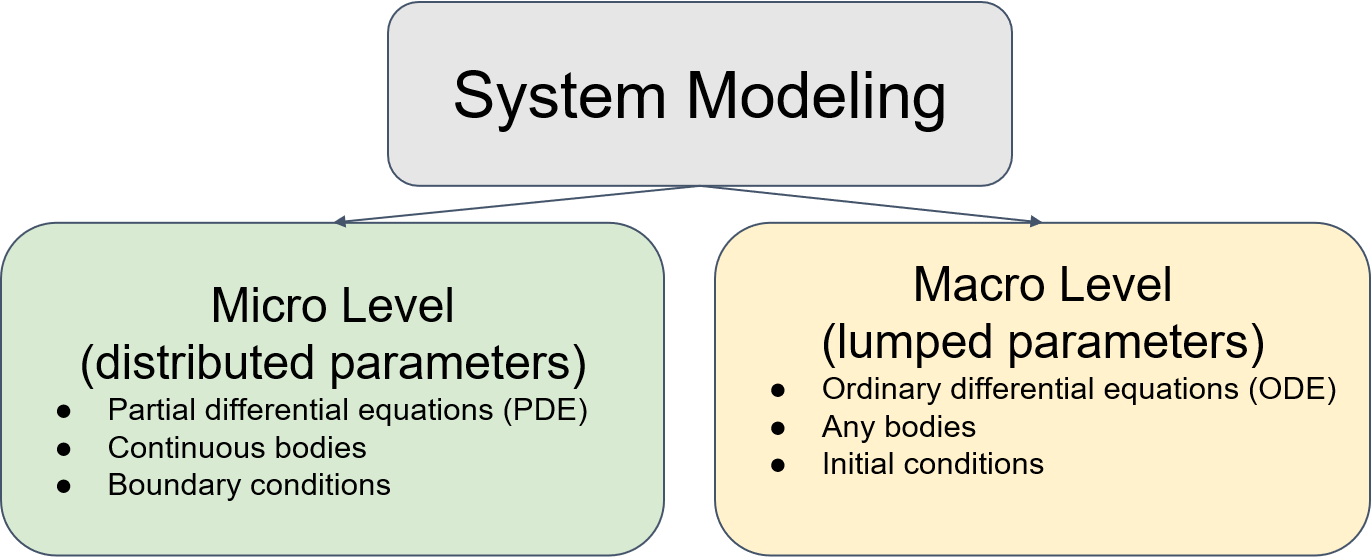
\includegraphics[height=6cm,width=1\textwidth,keepaspectratio]{system_modeling.png}
        \label{fig:system_modeling.png}
    \end{figure}
\end{frame}

\begin{frame}[t]{Common Methods}
    \framesubtitle{}
    \begin{columns}[T,onlytextwidth]
        \begin{column}{0.49\textwidth}
            \centering \textbf{Micro Level}
            \begin{itemize}
                \item Kek
            \end{itemize}
        \end{column}
        \begin{column}{0.49\textwidth}
            \centering \textbf{Macro Level}
            \begin{itemize}
                \item kukarec
            \end{itemize}
        \end{column}
    \end{columns}
\end{frame}

\begin{frame}[t]{Finite Difference Method}
    \framesubtitle{}

\end{frame}

\begin{frame}[t]{Finite Difference Method Material}
    \framesubtitle{}
    \scriptsize
    \begin{enumerate}
        \item \href{http://bigor.bmstu.ru/?cnt/?doc=Mkr/\%CA\%D0.mod/?cou=Mkr/base.cou}{Конечно-разностные аппроксимации производных (BIGOR)}
        \item \href{https://youtu.be/to82dv2SX28}{The Finite Difference Method (1D)}
        \item \href{https://www.youtube.com/watch?v=YotrBNLFen0}{Finite Differences}
        \item \href{https://www.youtube.com/watch?v=zSz-c4lFAuQ&t=5s}{РК6. Модели и методы анализа проектных решений. Метод конечных разностей, двумерные задачи}
        \item \href{https://youtu.be/gIOLPO16mEU}{Тихонов Н. А. - Основы математического моделирования - Метод конечных разностей (Лекция 7)}
        \item \href{https://youtu.be/DWCNVF9oMkw}{CODE Numerical Solution of 2D Laplace equation using Finite Difference Method}
        \item \href{https://youtu.be/Tfo12ylAMso}{Central Difference Approximation | Lecture 61 | Numerical Methods for Engineers}
        \item \href{https://www.youtube.com/watch?v=g3Xw1r7QGOE}{PDE | Finite differences: introduction}
        \item \href{https://youtu.be/FS6FcaX1O0U}{Оператор набла (оператор Гамильтона) и оператор Лапласа}
    \end{enumerate}
\end{frame}

\begin{frame}[t]{Finite Element Method}
    \framesubtitle{}

\end{frame}

\begin{frame}[t]{Finite Element Method (FEM)}
    \framesubtitle{Video}
    \vspace{-0.6cm}
    \begin{figure}[H]
        \href{https://youtu.be/GHjopp47vvQ}{
            \centering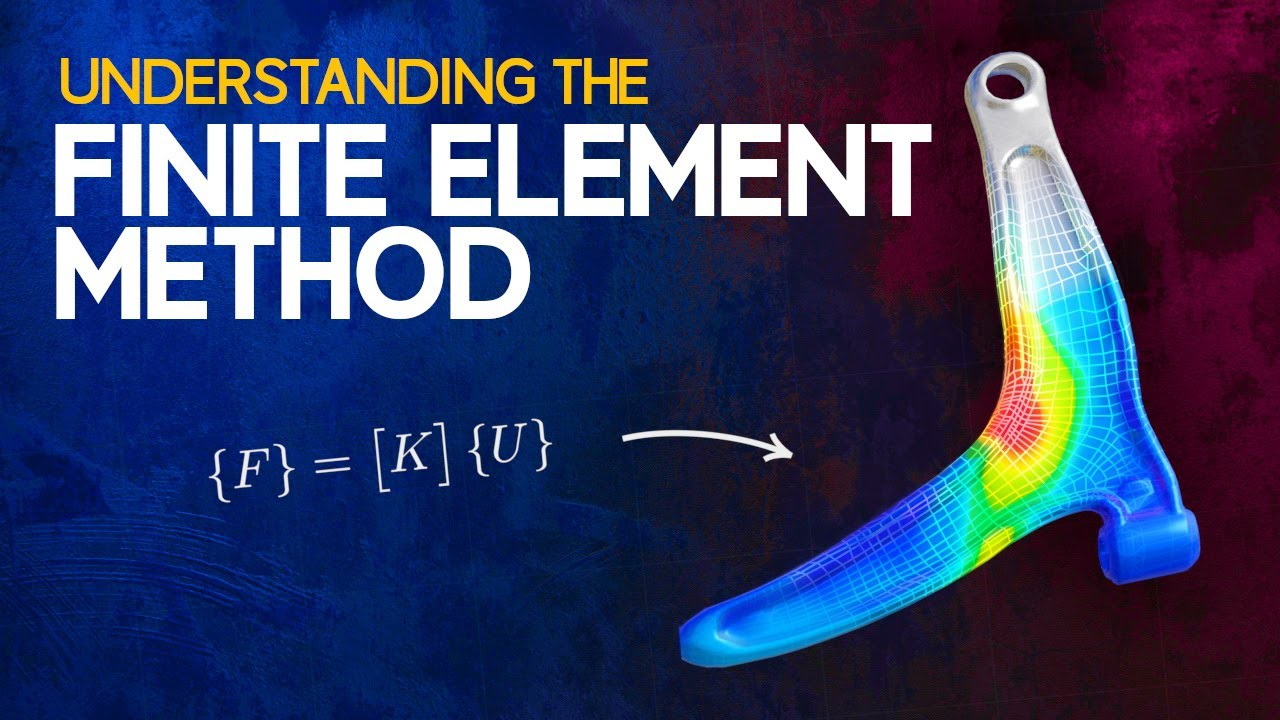
\includegraphics[height=6cm,width=1\textwidth,keepaspectratio]{fem_video.jpg}}
        \label{fig:fem_video.jpg}
    \end{figure}
\end{frame}

\begin{frame}[t]{Finite Element Method Materials}
    \framesubtitle{}
    \scriptsize
    \begin{enumerate}
        \item \href{http://bigor.bmstu.ru/?cnt/?doc=Mkr/id-fem.mod/?cou=Mkr/base.cou}{Идея метода конечных элементов (BIGOR)}
        \item \href{https://www.youtube.com/watch?v=W-llrHRydv8&list=PL0GvilEBvQdZH_PqDTilH9Hmp_--dWB33 }{Основы метода конечных элементов. Часть 1. Идея МКЭ в задачах конструкционного анализа}
        \item \href{https://www.youtube.com/watch?v=BA4iZtRfNxE&list=PLtaqFZsfPcLkas_BCVyqmVFGtNIzm9hg8&index=15}{РК6. Модели и методы анализа проектных решений. Метод конечных элементов: основные положения}
        \item \href{https://www.youtube.com/watch?v=KcrRM_22RjY}{РК6. Модели и методы анализа проектных решений. Метод конечных элементов: нестационарные задачи}
        \item \href{https://youtu.be/P4lBRuY7pC4}{Finite Element Method}
        \item \href{https://www.youtube.com/playlist?list=PL4__wpEQFpcjPZQ76CCcEmBaum5Iky4H3}{Метод конечных элементов. Основы 1.1}
        \item \href{https://www.youtube.com/playlist?list=PLnT2pATp7adU_OYwrPoDWE_YmePxu-fMf}{Finite Element Method in MATLAB}

    \end{enumerate}
\end{frame}

\begin{frame}[t]{Reference Materials}
    \framesubtitle{}
    \begin{enumerate}
        \item \href{https://youtu.be/p1AJqBWYEVE}{Метод конечных элементов (FEM) vs метод контрольного объёма (FVM). В чём разница?}
        \item \href{http://auts.samgtu.ru/sites/auts.samgtu.ru/files/upUSRP.pdf}{Математическое моделирование систем с распределёнными параметрами, книга}
        \item \href{http://bigor.bmstu.ru/?cnt/?doc=Mkr/base.cou}{Моделирование систем с распределенными параметрами (базовый курс) (BIGOR)}
        \item Muftu S. Finite Element Method: Physics and Solution Methods. --- Academic Press, 2022.
    \end{enumerate}
\end{frame}





\fbckg{fibeamer/figs/last_page.png}
\frame[plain]{}

\end{document}